\chapter{Description and operation of the product}\label{ch:description}

\section{Purpose}
The \ReplicaGenOne{} and \ReplicaNextLong{} dashboards replace the original Volkswagen instrument clusters while extending their functionality. They provide digital indications for speed, engine speed, coolant temperature, fuel level, and auxiliary MFA calculations, and they support both cable and electronic speed sensors. \ReplicaGenOneShort{} units integrate a Bluetooth controller, while \ReplicaNextShort{} adds Wi-Fi-based configuration modules and optional expansion units.

\section{Model identification}
Every dashboard is marked with a four-letter code that describes the drivetrain, assembly type, speed sensor interface, and wiring generation. Optional digits indicate the supported tachometer scale, and an additional three-letter suffix reports export measurement units.

\subsection{Four-letter designation}
\begin{description}
    \item[Position~1] \textbf{G} for petrol engines or \textbf{D} for diesel engines.
    \item[Position~2] \textbf{A} for factory-assembled units or \textbf{M} for self-assembly kits.
    \item[Position~3] \textbf{C} for a mechanical cable speed sensor or \textbf{R} for an electronic speed sensor.
    \item[Position~4] \textbf{T} for the pre-facelift (CE~1) harness or \textbf{S} for the facelift (CE~2) harness.
\end{description}
A trailing digit denotes the maximum displayed engine speed in thousands of RPM (for example, “8” on a GACT8 cluster equals an 8000~RPM scale).

\subsection{Measurement suffix}
Export variants may add a three-letter suffix formed from the set \texttt{MGFK}:
\begin{description}
    \item[M] miles per hour,
    \item[G] gallons,
    \item[F] Fahrenheit,
    \item[K] Kelvin.
\end{description}
For example, a \texttt{GART8-MGF} dashboard is a petrol, factory-assembled, electronic-sensor, CE~2 unit with an 8000~RPM tachometer and imperial measurement units.

\section{Model range}
{\scriptsize
\begin{tblr}{
    colspec={Q[l,2.2cm] X[l]},
    hlines
}
\textbf{Model} & \textbf{Description} \\
GACT & Petrol, fully assembled, cable speed sensor, two connectors, 7000~RPM scale. \\
GART & Petrol, fully assembled, remote electronic speed sensor, two connectors, 7000~RPM scale. \\
GAC & Petrol, fully assembled, cable speed sensor, single connector, 7000~RPM scale. \\
GARS & Petrol, fully assembled, remote electronic speed sensor, single connector, 7000~RPM scale. \\
GACT8 & Petrol, fully assembled, cable speed sensor, two connectors, 8000~RPM scale. \\
GART8 & Petrol, fully assembled, remote electronic speed sensor, two connectors, 8000~RPM scale. \\
GACS8 & Petrol, fully assembled, cable speed sensor, single connector, 8000~RPM scale. \\
GARS8 & Petrol, fully assembled, remote electronic speed sensor, single connector, 8000~RPM scale. \\
DACT & Diesel, fully assembled, cable speed sensor, two connectors, 6000~RPM scale. \\
DART & Diesel, fully assembled, remote electronic speed sensor, two connectors, 6000~RPM scale. \\
DACS & Diesel, fully assembled, cable speed sensor, single connector, 6000~RPM scale. \\
DARS & Diesel, fully assembled, remote electronic speed sensor, single connector, 6000~RPM scale. \\
MT & Self-assembly kit with two connectors. \\
M.S. & Self-assembly kit with a single connector. \\
NEXT-GART & \ReplicaNextLong{}, 8000~RPM scale, two connectors, electronic speed sensor. \\
NEXT-GARS & \ReplicaNextLong{}, 8000~RPM scale, single connector, electronic speed sensor. \\
NEXT-MT & \ReplicaNextLong{} self-assembly kit with two connectors. \\
NEXT-MS & \ReplicaNextLong{} self-assembly kit with a single connector. \\
\end{tblr}}

\section{Connector pin-outs}
\subsection{Clusters with two connectors}
\begin{figure}[htbp]
    \centering
    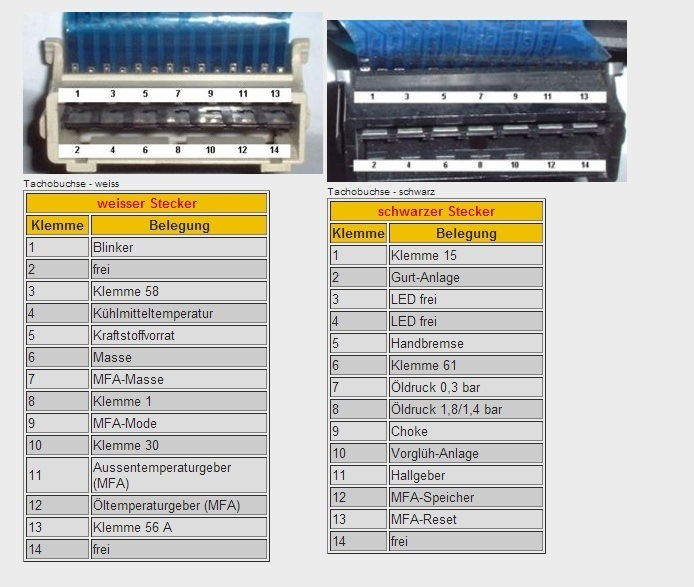
\includegraphics[width=0.72\textwidth]{digifiz_manual/image008.jpg}
    \caption{Connector layout for dual-connector \ReplicaGenOne{} dashboards.}
\end{figure}

\noindent\textbf{White connector}

{\scriptsize
\begin{tblr}{
    colspec={Q[l,1.4cm] X[l]},
    hlines
}
\textbf{Pin} & \textbf{Assignment} \\
1 & Blinker output, tied to ground for the indicator lamp. \\
2 & Frei --- not connected. \\
3 & Terminal~58, positive supply for the panel backlight. \\
4 & Resistive coolant temperature sensor input. \\
5 & Resistive fuel level sensor input. \\
6 & Ground return. \\
7 & Additional ground return. \\
8 & Terminal~1 engine-speed signal (coil, distributor, or other waveform up to 12~V with possible 300~V spikes). \\
9 & MFA mode line used to change MFA functions. \\
10 & UNR permanent positive supply (unused on \ReplicaGenOneShort{}, main supply on \ReplicaNextShort{}). \\
11 & MFA temperature “+” lead for the ambient sensor (\ReplicaNextShort{}). \\
12 & MFA oil temperature sensor lead (\ReplicaNextShort{} only). \\
13 & KL~56a high-beam indicator input (+12~V active). \\
\end{tblr}}

\noindent\textbf{Black connector}

{\scriptsize
\begin{tblr}{
    colspec={Q[l,1.4cm] X[l]},
    hlines
}
\textbf{Pin} & \textbf{Assignment} \\
1 & Terminal~15 switched +12~V from the ignition switch. \\
2--4 & Not connected. \\
5 & Handbrake indicator input (active low). \\
6 & KL~61 generator warning lamp drive with 120~\ensuremath{\Omega} excitation resistor. \\
7 & Oil pressure switch, 0.3~bar. \\
8 & Oil pressure switch, 1.8~bar. \\
9 & Not used. \\
10 & Glow-plug indicator input (+12~V active, diesel only). \\
11 & Hall sensor input for optional speed sensors. \\
12 & MFA block selection line. \\
13 & MFA reset line. \\
\end{tblr}}

\subsection{Clusters with a single connector}
Single-connector dashboards use the mapping shown in \autoref{fig:single-connector}. The harness replicates the same signals found on the dual-connector variants but consolidates them into a single plug.

\begin{figure}[htbp]
    \centering
    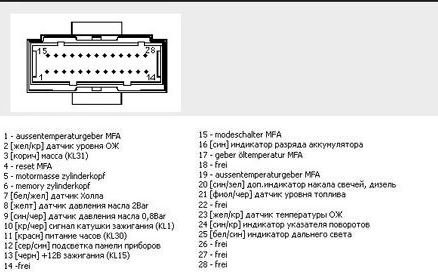
\includegraphics[width=0.65\textwidth]{digifiz_manual/image009.png}
    \caption{Single-connector layout used on compact Replica dashboards.}
    \label{fig:single-connector}
\end{figure}

\subsection{Scirocco/Passat prospective harness}
The prospective Scirocco/Passat harness uses two plugs. Their functions are summarised below.

\noindent\textbf{5-pin plug}
{\scriptsize
\begin{tblr}{
    colspec={Q[l,2.6cm] X[l]},
    hlines
}
\textbf{Pin} & \textbf{Assignment} \\
1~(D3) & Automatic-transmission “D” range indicator contact. Grounds the drive lamp when the selector is in position~D. \\
2~(D2) & Automatic-transmission second-range indicator contact. Grounds the “2” lamp when the selector is in position~2. \\
3~(D1) & Automatic-transmission low-range indicator contact. Grounds the “1” lamp when the selector is in position~1. \\
4~(SA) & Common feed for the automatic selector display (\emph{Schaltanzeige}); provides the +12~V supply for the range lamps. \\
5~(SPERRE) & Starter interlock contact from the selector. Closed in park or neutral to permit engine cranking. \\
\end{tblr}}

\noindent\textbf{14-pin plug}
{\scriptsize
\begin{tblr}{
    colspec={Q[l,2.6cm] X[l]},
    hlines
}
\textbf{Pin} & \textbf{Assignment} \\
1~(KL~58) & Illumination supply for the panel backlight. \\
2~(MASS) & Chassis ground return. \\
3~(TANK) & Fuel-level sender input. \\
4~(TEMP) & Coolant temperature sender input. \\
5~(KL~1) & Engine-speed signal (terminal~1). \\
6~(UHR) & Permanent +12~V feed for the clock and memory backup. \\
7~(FERNL) & High-beam indicator input. \\
8~(reserved) & Not connected. \\
9~(OEL~1.8) & High-pressure oil switch, 1.8~bar. \\
10~(CAT~VORGL(-)) & Catalytic-preheat / diesel pre-glow warning lamp input (active low). \\
11~(OEL~0.3) & Low-pressure oil switch, 0.3~bar. \\
12~(KL~61) & Alternator warning lamp and excitation feed. \\
13~(KL~49a) & Combined turn-signal indicator feed. \\
14~(KL~15) & Ignition-switched +12~V supply. \\
\end{tblr}}

\subsection{Mk1 connector mapping}
Volkswagen Mk1 vehicles use the following assignments:
\begin{enumerate}
    \item Illumination and low-beam supply.
    \item MASSE~31 ground reference.
    \item TANK fuel-level sender.
    \item TEMP coolant temperature sender.
    \item KL~1 tachometer signal.
    \item UHR permanent +12~V.
    \item KL~56 high-beam signal.
    \item OIL (HIGH) 1.8~bar pressure switch.
    \item OIL (LOW) 0.3~bar pressure switch.
    \item Diesel glow indicator.
    \item CHOKE input (unused).
    \item KL~61 generator lamp.
    \item Blinker input (combined left/right).
    \item KL~15 ignition supply.
\end{enumerate}
\begin{figure}[htbp]
    \centering
    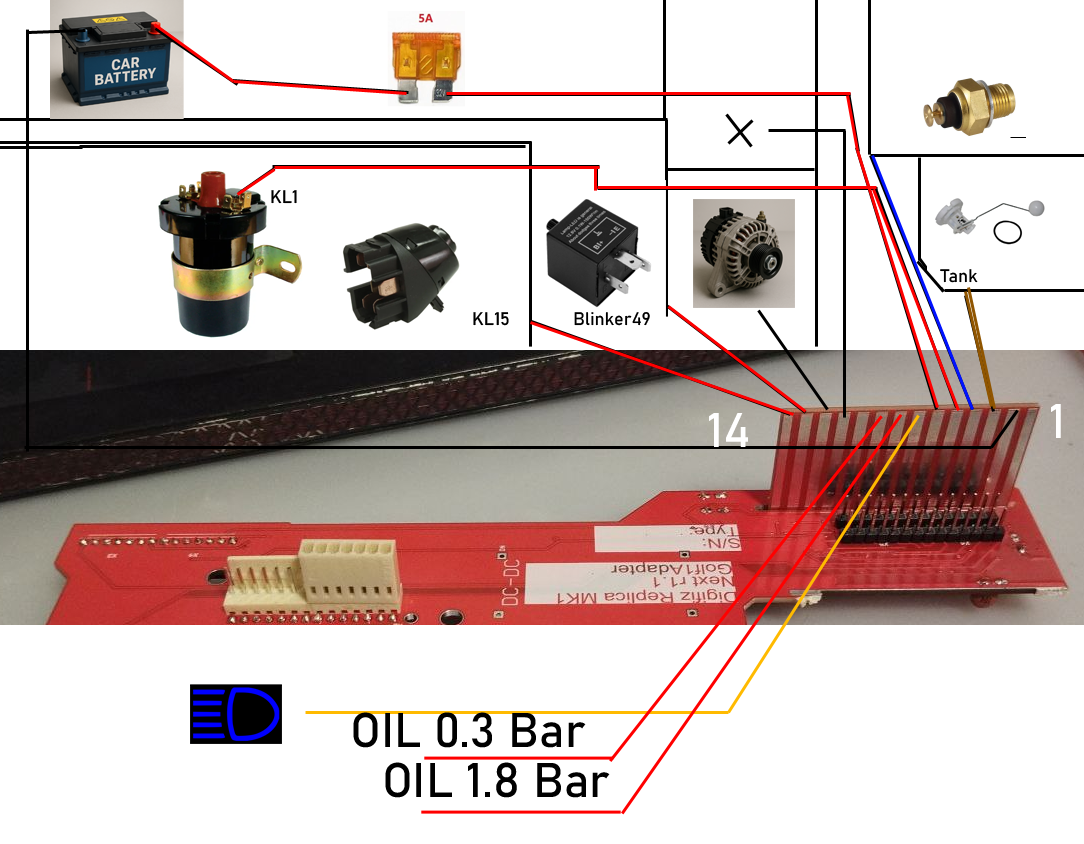
\includegraphics[width=0.75\textwidth]{digifiz_manual/image010.png}
    \caption{Harness connection diagram for Mk1 installations.}
\end{figure}

\subsection{Printed-circuit-board service connector}
The third connector on the circuit board mirrors the dashboard connectors, with pins numbered right-to-left on \ReplicaGenOneShort{} and \ReplicaNextShort{} units. It provides a service interface with the assignments listed in \autoref{tab:service-connector}.

\begin{table}[htbp]
    \centering
    \caption{Service connector pin assignments.}
    \label{tab:service-connector}
    {\scriptsize
    \begin{tblr}{
        colspec={Q[l,1.9cm] X[l]},
        hlines,
    }
        \textbf{Position} & \textbf{Assignment} \\
        1 & Indicator output. \\
        2 & Speed sensor input (SPM\_M). \\
        3 & Vehicle ground. \\
        4 & Indicator output. \\
        5 & Left blinker optocoupler input. \\
        6 & Right blinker optocoupler input. \\
        7 & Ignition +12~V. \\
        8 & Diesel-specific input. \\
        9 & Indicator input (positive). \\
        10 & Alternative RPM input (unused, \ReplicaNextShort{} only). \\
        11 & \ReplicaGenOneShort{}: indicator output (normally disconnected); \ReplicaNextShort{}: brake input (active low). \\
        12 & Reserved. \\
        13 & Check-engine input. \\
        14 & No contact. \\
    \end{tblr}}
\end{table}

\subsection{Auxiliary expansion connectors}
Three supplementary four-pin headers are fitted to the main board to simplify harness upgrades and service work:
\begin{itemize}
    \item \textbf{Expansion analog signals:} provides a dedicated breakout for additional analog inputs when integrating custom sensors.
    \item \textbf{MFA mirror:} duplicates the standard \textsc{MFA} connector to support parallel tapping of the trip computer signals.
    \item \textbf{Analog duplicates:} repeats the oil temperature, ambient temperature, and brake indicator inputs so these circuits can be routed to external logging or monitoring modules.
\end{itemize}
All three use the \mbox{KF2510-4p} mating connector, which is not supplied with the dashboard kit and must be sourced separately if needed.

\begin{figure}[htbp]
    \centering
    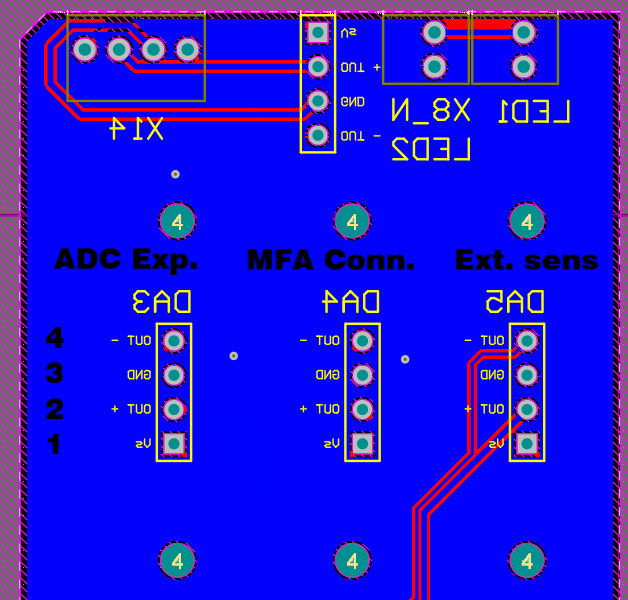
\includegraphics[width=0.6\textwidth]{digifiz_manual/ext_conn.png}
    \caption{Auxiliary connector layout on the main board.}
\end{figure}

\begin{table}[htbp]
    \centering
    {\small
    \begin{tblr}{
        colspec={Q[l,2.3cm] Q[c,1.3cm] X[l]},
        hlines,
        row{1} = {font=\bfseries}
    }
    Connector & Pin & Assignment \\
    Connector~I & 4 & Aux analog input~1 \\
    Connector~I & 3 & Ground (GND) \\
    Connector~I & 2 & Aux analog input~2 \\
    Connector~I & 1 & VCC (3V3, unfused\textbf{!!!}) \\
    Connector~II & 4 & MFA reset \\
    Connector~II & 3 & Ground (GND) \\
    Connector~II & 2 & MFA memory block \\
    Connector~II & 1 & MFA mode \\
    Connector~III & 4 & Oil temperature sensor output \\
    Connector~III & 3 & Ground (GND) \\
    Connector~III & 2 & Outdoor temperature sensor output \\
    Connector~III & 1 & Brake indicator \\
    \end{tblr}}
    \caption{Pin assignments for the auxiliary expansion connectors.}
\end{table}

\section{Embedded software and completeness}
The dashboard firmware is published at the following address:
\displayurl{https://github.com/Sgw32/DigifizReplica}
Two delivery sets are available:
\begin{itemize}
    \item \textbf{\ReplicaGenOne{}:} dashboard assembly, ambient and oil temperature harness, USBasp programmer, and (for remote sensors) a speed sensor harness.
    \item \textbf{\ReplicaNextLong{}:} dashboard assembly and an electronic speed sensor harness.
\end{itemize}
